\subsection{Completed Labeled-Only Physical-Structure Panel}

All 24 new structure models and three reused X3 CE references complete the registered seven-view protocol. The source/input binding repair and the device-only WRONG\_REFERENCE replacement are applied before aggregation; failed historical outputs are excluded. This panel uses matched CE, satellite weight 0.68, no label smoothing, CRIC, KL, U, or EMA, and 50 epochs/11,100 updates per F. It is separate from the native T1 method and the historical single-view E200 architecture study.

\begin{table*}[t]\centering\footnotesize\caption{Strict L-only architecture results (mean$\pm$sample SD over three F seeds, conditional on one G-L). Six-view means are formed within each seed. X3$-$variant is paired; positive values favor X3. Deletions can alter capacity and computation.}\label{tab:structure-complete}\begin{tabular}{lrrrrr}\toprule

Structure & Raw clean (\%) & Raw six (\%) & G-L six (\%) & G-L six Macro-F1 (\%) & X3$-$variant (pp)\\\midrule

X3\_CE & $81.55\pm1.34$ & $46.35\pm1.74$ & $74.49\pm1.14$ & $73.91\pm1.29$ & ---\\

SIG\_TIME & $81.82\pm1.26$ & $43.61\pm6.18$ & $74.20\pm1.16$ & $73.72\pm1.33$ & $0.284\pm0.367$\\

NO\_TIME & $80.95\pm1.54$ & $45.46\pm5.89$ & $73.99\pm1.03$ & $73.39\pm1.27$ & $0.499\pm0.150$\\

NO\_SIGNATURE & $79.48\pm1.72$ & $41.84\pm5.75$ & $72.32\pm1.09$ & $71.92\pm1.09$ & $2.172\pm0.106$\\

NO\_PA & $78.94\pm2.29$ & $39.39\pm5.78$ & $71.70\pm0.44$ & $71.13\pm0.49$ & $2.792\pm0.856$\\

NO\_REFERENCE & $78.64\pm1.49$ & $44.80\pm2.93$ & $73.01\pm1.15$ & $72.32\pm1.16$ & $1.478\pm0.008$\\

COV\_X3 & $81.69\pm0.61$ & $49.36\pm4.72$ & $74.56\pm0.84$ & $73.89\pm0.89$ & $-0.067\pm0.659$\\

SHUFFLE\_TIME & $82.20\pm1.72$ & $48.54\pm6.44$ & $75.62\pm1.11$ & $75.10\pm1.24$ & $-1.133\pm0.769$\\

WRONG\_REFERENCE & $81.02\pm1.20$ & $46.59\pm2.91$ & $74.24\pm1.09$ & $73.64\pm1.24$ & $0.250\pm0.216$\\

\bottomrule\end{tabular}\end{table*}

The PA, sequence-residual and known-excitation-response deletions reduce restored six-view accuracy by $2.792\pm0.856$, $2.172\pm0.106$ and $1.478\pm0.008$ pp, respectively. The equal-parameter no-time and wrong-reference controls yield smaller paired differences ($0.499\pm0.150$ and $0.250\pm0.216$ pp). However, shuffled time exceeds X3 after G-L by $1.133\pm0.769$ pp, and covariance X3 is slightly higher on average. These outcomes do not establish that the original sequence ordering is essential or that every physical prior improves recognition. Raw sensitivity and restored performance are reported separately.

\begin{figure*}[t]\centering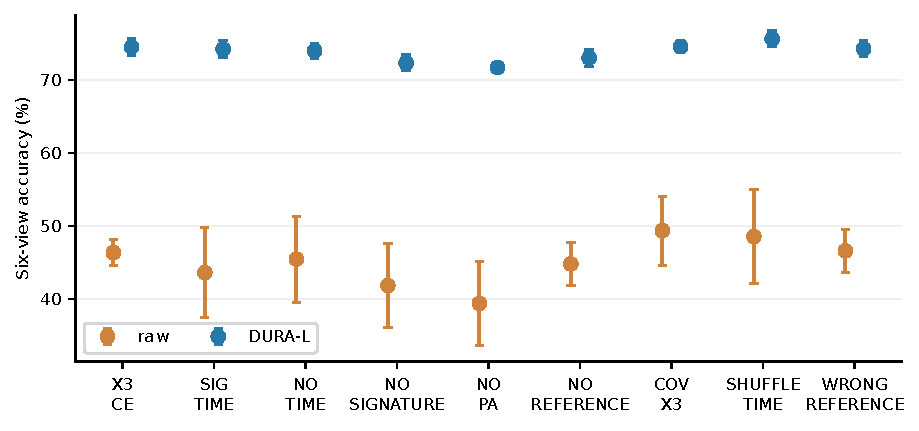
\includegraphics[width=.92\textwidth]{images/final_panels/structure_accuracy.pdf}\caption{Matched strict-CE structure controls. Error bars are three-F-seed SD, not significance intervals.}\label{fig:structure-accuracy}\end{figure*}

All 27 source diagnostics use the same 720 labeled packets across 90 TX/RX/day strata and 11 fixed interventions, with zero U/target reads or probe updates. The source geometry margin does not rank target accuracy: deleting the sequence-residual branch increases the source margin while reducing restored recognition. Fixed interventions therefore characterize sensitivity and inductive bias; they do not recover hardware parameters or prove complete receiver/channel disentanglement. Synthetic PA perturbations are not assumed identity-preserving.

\begin{figure*}[t]\centering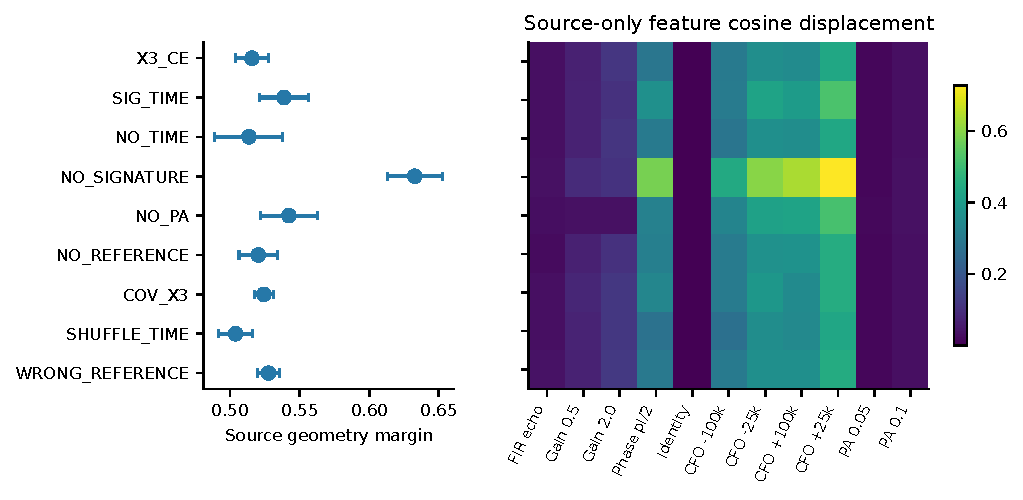
\includegraphics[width=.94\textwidth]{images/final_panels/structure_physics.pdf}\caption{Source-only geometry and deployed-feature response to fixed interventions; no probe fitting or target optimization.}\label{fig:structure-physics}\end{figure*}

The 24 new F models require 17.813 shared-worker elapsed hours across 72 source stages (1200 model epochs, 266400 updates). The three CE references reuse 2.148 historical hours. These are neither isolated GPU hours nor new end-to-end wall time; shared G-L ancestry is reported once separately.

\subsection{Restoration Transfer to Four External Classifiers}

All 516 existing external F models now have raw, same-contract G-L and G-LU readouts (1548 cells before views/tasks), with no additional F/G training. All declared predictions are frozen before independent scoring. We reconstruct 516600 serialized confusion matrices, including RX/TX/day strata, and preserve the chronological auxiliary task. ManyRx uses ten classes; the other contracts use six. The 34 FP32 restored-IQ caches contain no labels or classifier outputs and do not renormalize the locked received-IQ observations.

\begin{table*}[t]\centering\footnotesize\caption{F0 external classifiers after restoration. Each row retains its native training budget and jointly trained default head. Sup+G-L alone is fully L-only; PL uses U through F, and G-LU uses U through restoration. Means$\pm$SD are over three F seeds conditional on fixed G.}\label{tab:external-DURA-complete}\begin{tabular}{lllrrrr}\toprule

Method & Objective & F regime & Raw clean (\%) & Raw six (\%) & G-L six (\%) & G-LU six (\%)\\\midrule

RIEI & CE & Sup & $66.50\pm1.37$ & $53.12\pm0.89$ & $62.52\pm1.32$ & $62.80\pm1.50$\\

RIEI & FULL & Sup & $54.53\pm8.31$ & $47.68\pm6.42$ & $49.33\pm6.36$ & $49.11\pm6.13$\\

RIEI & CE & PL & $66.45\pm1.37$ & $53.00\pm0.97$ & $62.55\pm1.19$ & $62.82\pm1.36$\\

RIEI & FULL & PL & $53.53\pm6.48$ & $47.50\pm5.66$ & $48.55\pm5.11$ & $48.22\pm4.86$\\

DRIFT-v2 & CE & Sup & $68.49\pm2.50$ & $34.19\pm4.33$ & $64.82\pm3.02$ & $65.54\pm3.23$\\

DRIFT-v2 & FULL & Sup & $67.33\pm5.91$ & $26.83\pm3.36$ & $62.01\pm6.30$ & $62.50\pm5.68$\\

DRIFT-v2 & CE & PL & $70.50\pm3.78$ & $31.07\pm6.99$ & $65.03\pm4.24$ & $65.47\pm4.65$\\

DRIFT-v2 & FULL & PL & $60.97\pm11.26$ & $27.28\pm3.11$ & $55.81\pm8.46$ & $56.57\pm9.42$\\

IB-RFF & CE & Sup & $63.30\pm2.14$ & $18.04\pm2.31$ & $61.04\pm2.11$ & $59.70\pm2.08$\\

IB-RFF & FULL & Sup & $63.77\pm2.18$ & $15.78\pm4.87$ & $61.43\pm1.98$ & $60.72\pm1.85$\\

IB-RFF & CE & PL & $64.78\pm3.20$ & $17.79\pm0.81$ & $63.46\pm2.63$ & $62.28\pm3.04$\\

IB-RFF & FULL & PL & $66.08\pm0.99$ & $18.44\pm4.30$ & $63.81\pm0.85$ & $63.66\pm0.96$\\

SDG & CE & Sup & $73.73\pm0.91$ & $35.15\pm5.17$ & $67.89\pm1.73$ & $67.30\pm1.79$\\

SDG & FULL & Sup & $71.39\pm1.84$ & $58.14\pm2.32$ & $65.22\pm1.85$ & $65.52\pm2.24$\\

SDG & CE & PL & $72.01\pm2.78$ & $42.02\pm5.37$ & $65.91\pm2.13$ & $65.56\pm2.08$\\

SDG & FULL & PL & $72.10\pm0.41$ & $58.15\pm1.53$ & $65.57\pm0.52$ & $66.18\pm0.21$\\

\bottomrule\end{tabular}\end{table*}

Across the declared main-task method/recipe/contract/restorer conditions, 4/344 restored-minus-raw six-view means and 192/344 clean means are nonpositive. Full-minus-own-CE is nonpositive in 148/258 six-view conditions. These condition counts are not independent dataset replications or significance tests. Negative effects, nonmonotonic curves and zero ordinary-PL acceptance remain in the analysis.

\begin{figure*}[t]\centering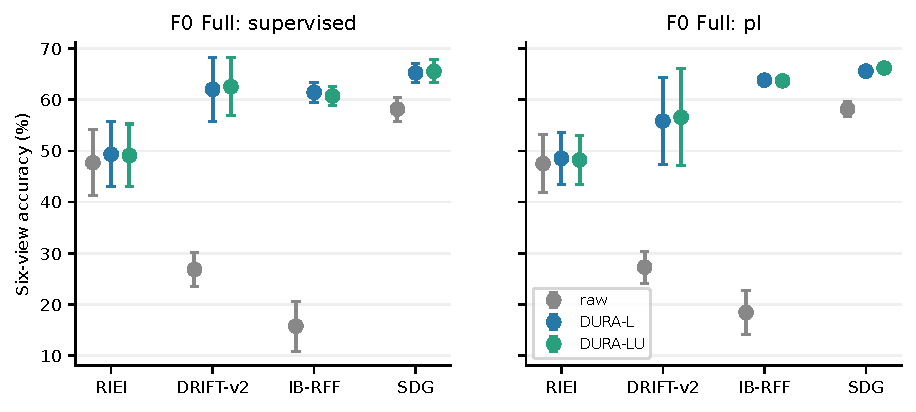
\includegraphics[width=.91\textwidth]{images/final_panels/external_F0.pdf}\caption{Frozen external Full classifiers with raw and matched L/LU restoration on F0. Restoration helps some classifiers substantially and does not uniformly improve all methods or clean views.}\label{fig:external-F0}\end{figure*}

Source-count curves retain $m=1,2,3,4,6$ with exactly six target RX/144000 packets. F0 has seven target RX/168000 packets and is not an $m=5$ curve point. Natural supervised, natural ordinary-PL and fixed-L/V supervised curves are exported separately, including own-CE controls. The dashed PAMF line uses the matching supervised or ordinary-PL recipe and the same G-LU permission; native selective T1 SSL remains a separate method. Chronological all-date aggregates are not labeled future generalization; D3 and source-RX unseen-date diagnostics retain their own strata.

\begin{figure*}[t]\centering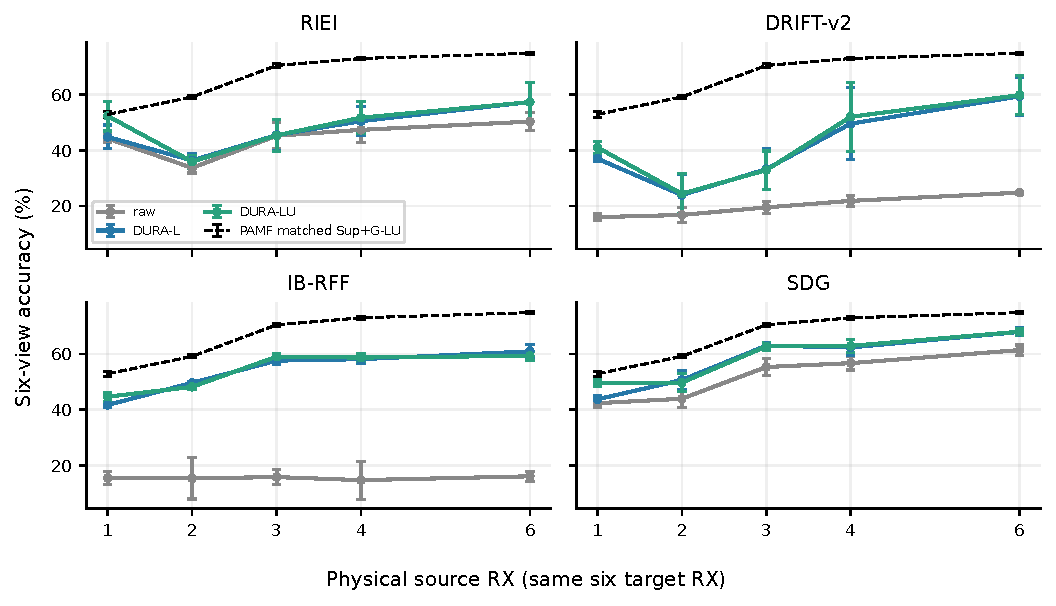
\includegraphics[width=.92\textwidth]{images/final_panels/external_source_natural_supervised.pdf}\caption{Natural-budget supervised source-count curves after frozen restoration. Each panel retains its method-native budget; the PAMF matched Sup+G-LU reference uses the same six-target contract. Error bars: three-F-seed SD.}\label{fig:external-source}\end{figure*}

The 654 original F-stage records retain selection, epochs, updates, augmentation and PL exposures. Shared G ancestry, one-time restored-IQ generation, cached classification and CPU scoring costs are separated. Cache classification time is not an online G+F latency measurement. The already completed concatenation/0.68-gradient audit is reused; no external classifier is retrained.

\subsection{Ordinary-PL and G-Data-Permission Factorial}

The 51 added PL-F/G-L predictions close 204 cells over 17 contracts, three F seeds and the four combinations of supervised/ordinary-PL F with L/LU G. Raw decisions are exactly reused for each F. Native selective T1 SSL is excluded from this ordinary-PL factorial. All within-seed task/view aggregates precede paired contrasts and three-seed summaries.

\begin{table}[t]\centering\footnotesize\caption{F0 data-permission factorial (six-view accuracy). Only Sup+G-L is a fully L-only system.}\label{tab:gfactor-complete}\begin{tabular}{lr}\toprule Cell & Mean$\pm$SD (\%)\\\midrule

Sup+G-L & $76.837\pm0.531$\\

Sup+G-LU & $77.777\pm0.275$\\

PL+G-L & $76.704\pm0.662$\\

PL+G-LU & $77.613\pm0.369$\\

\bottomrule\end{tabular}\end{table}

On F0, PL-minus-Sup is $-0.134\pm0.551$ pp with G-L and $-0.165\pm0.134$ pp with G-LU. G-LU-minus-G-L is $0.940\pm0.367$ pp at Sup and $0.909\pm0.295$ pp at PL. The paired difference-in-differences is $-0.031\pm0.420$ pp. These results do not establish positive PL/restoration synergy. Effects vary across contracts, including negative G-U contributions on the chronological aggregate. SD is not a significance test.

\begin{figure*}[t]\centering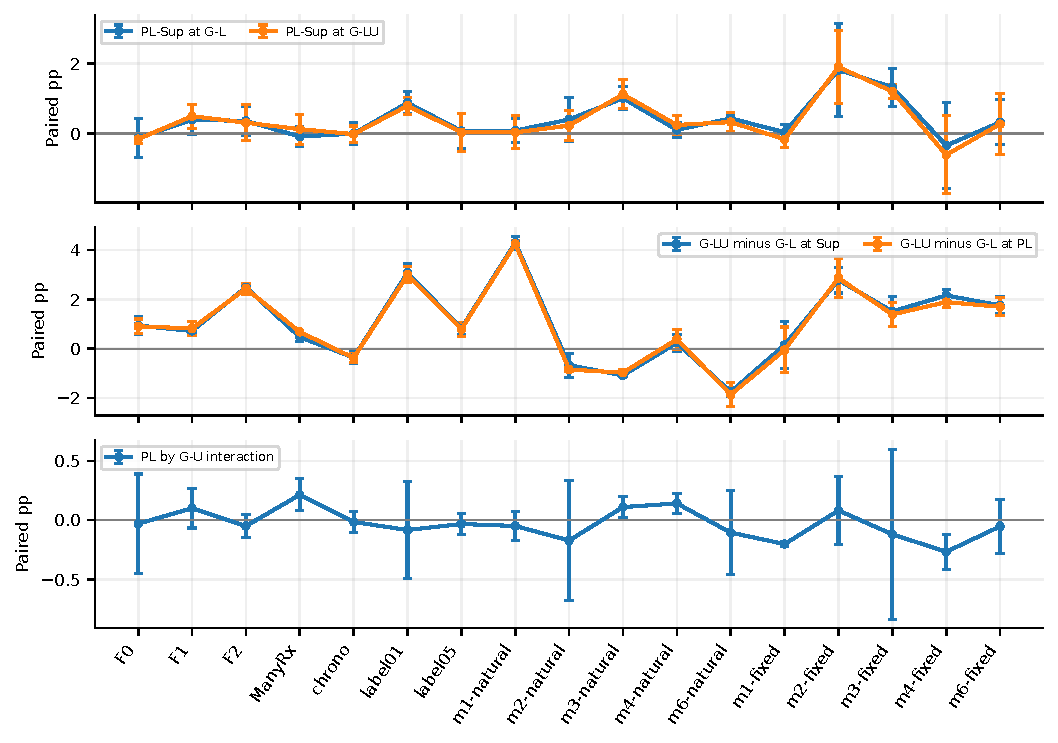
\includegraphics[width=.92\textwidth]{images/final_panels/gfactor_effects.pdf}\caption{Permission-factorial paired effects across all registered contracts. The chronology main aggregate covers all dates; its D3 future endpoint remains separately available. Error bars are three-F-seed SD.}\label{fig:gfactor-effects}\end{figure*}

\subsection{Completed Dedicated Mechanism Timing}

The two source-only adjunct panels finish on exclusive RTX3090 GPUs 5 and 1, excluding GPUs 2/3. The corrected-F/G panel covers 36 cases by five batch sizes by five rounds (900 case-rounds, 252000 GPU-wall and 18000 CPU-return calls); the strict-structure panel covers 18 cases (450 case-rounds, 126000 GPU-wall and 9000 CPU-return calls). Each uses fixed seed01 weights, FP32/TF32 off, batch sizes 1/8/32/64/128, and two CPU threads. Five timing rounds are not five model seeds. Every round median/P95 is independently reconstructed from its samples.

\begin{table}[t]\centering\footnotesize\setlength{\tabcolsep}{4pt}\caption{Dedicated strict-structure B1 timing (ms). F-only is eager; G-L+F uses Graphs and residual reuse. These execution routes differ.}\label{tab:structure-timing}\begin{tabular}{lrrr}\toprule Structure & F eager & G-L+F & G-L+F P95\\\midrule

X3\_CE & 7.328 & 4.559 & 4.615\\

SIG\_TIME & 6.650 & 4.496 & 4.528\\

NO\_TIME & 7.475 & 4.555 & 4.614\\

NO\_SIGNATURE & 6.300 & 4.461 & 4.562\\

NO\_PA & 6.012 & 4.389 & 4.462\\

NO\_REFERENCE & 5.869 & 4.422 & 4.449\\

COV\_X3 & 7.101 & 4.526 & 4.555\\

SHUFFLE\_TIME & 7.318 & 4.551 & 4.574\\

WRONG\_REFERENCE & 7.371 & 4.554 & 4.601\\

\bottomrule\end{tabular}\end{table}

G-student mechanism timings use eager G (and eager F for G+F); they must not be interpreted as residual-reuse/Graph speedups. Corrected F06--F10 use eager F-only and the locked optimized G+F route. Their complete batch, P95, CPU-return, five-round dispersion, operator and incremental-allocation tables are exported. Absolute resident memory contains all benchmark models and Graph pools; it is not isolated single-model VRAM. Deployment parameter counts exclude the larger training wrapper. First-call values follow loading/profiling, not fresh-process startup.

The previously delivered uniform latency-r02 result remains the official final T1 default: B1 median 4.541187ms, P95 4.725135ms, and CPU class return 4.611311ms. It is not remeasured or replaced by these adjunct panels. The sole historical RIEI-import timing failure remains recorded and explicitly substituted by r02; the terminal controller label can therefore retain PARTIAL\_TECHNICAL\_FAILURE while every effective scientific phase is closed.

All current declared training, frozen prediction, independent scoring and timing phases are complete. Unpublished fine-control training and its additional proposed timing rounds remain explicitly deferred, rather than fabricated as completed evidence. No target result changes defaults, parameters, selection, queues or reruns.
